%%=============================================
% !Mode:: "TeX:UTF-8"
% !TEX program  = XeLaTeX
%%=============================================
% 模板名称:hitszthesis
% 模板版本:V3.0.3
% 模板作者:杨敬轩(Jingxuan Yang)
% 联系作者:yangjingxuan@stu.hit.edu.cn & yanglatex2e@gmail.com
% 模板交流:QQ群:1039392552,加群请备注LaTeX、hitszthesis相关说明
% 模板适用:哈尔滨工业大学(深圳)本、硕、博学位论文
% 模板编译:手动编译方法参看 README.md 或 hitszthesis.pdf
%          GNU make 工具:make thesis
%          Windows批处理脚本:双击 compile.bat 自动编译论文
%          更多编译细节详见说明文档:hitszthesis.pdf
% 更新时间:2020/03/12
% 模板帮助:请**务必务必务必**阅读 hitszthesis.pdf 说明文档,文档查看方法:
%          cmd 命令行:texdoc hitszthesis
%          推荐前往模板的 GitHub 仓库获取最新文件,地址:
%          https://github.com/YangLaTeX/hitszthesis
%%=============================================

% 设置文档类别为 <hitszthesis>,本文档为本科毕业设计(论文)的示例
\documentclass[type=bachelor,infoleft=true]{hitszthesis}

% 模板提供以下选项,各个选项之间不要有空格
% 1. type=bachelor|master|doctor
%   含义:本科、硕士、博士学位论文,不设默认值,**必填**
% 2. covertitletworow=true|false
%   含义:本科封面第一页标题单行或多行显示,默认为单行显示(false)
% 3. infoleft=true|false
%   含义:本科封面第二页下划线内容居中或居左显示,默认为居中显示(false)
% 4. mathfont=newtxmath|mtprotwolite|mtprotwo
%   含义:正文数学字体选项:newtxmath(默认),mtprotwolite(lite版,免费),
%         mtprotwo(完全版,需购买授权),
%         mtpro2字体官网:https://www.pctex.com/mtpro2.html
% 5. boldcaption=true|false
%   含义:图表题注是否加粗,默认为不加粗(false)
% 6. tocfour=true|false
%   含义:是否添加第四级目录,只对本科文科个别要求四级目录有效,默认不添加(false)
% 7. fulltime=true|false
%   含义:是否全日制,非全日制如同等学力等,要在coverinformation中设置类型,
%        默认是全日制(true)
% 8. subtitle=true|false
%   含义:论文题目是否含有副标题,默认没有副标题(false)
% 9. openright=true|false
%   含义:博士论文是否要求章节首页必须在奇数页,默认否(false)
% 10. library=true|false
%   含义:是否为提交到图书馆的电子版,默认否(false)

% 自定义设置与额外加载的宏包请写在 \file{hitszthesis.sty} 里
\usepackage{hitszthesis}

% 图片存放路径,在这些文件夹里的图片可以直接使用图片文件名调用
\graphicspath{{figures/}{pictures/}}

%%=============================================
% 开始写论文
% !!注意本文仅作为排版格式示例,并不作为毕业论文规范
\begin{document}

% 若题目过长,则需使用以下命令调整本科封面第二页下划线长度
%\infowidth = 9cm

% 开始写前言部分
\frontmatter

% 封面信息填写
% !TEX root = ../main.tex

\hitszsetup{
  %******************************
  % 注意:
  %   1. 配置里面不要出现空行
  %   2. 不需要的配置信息可以删除
  %******************************
  %
  %=====
  % 秘级
  %=====
  statesecrets={公开},
  natclassifiedindex={TM301.2},
  intclassifiedindex={62-5},
  %
  %=========
  % 中文信息
  %=========
  ctitleone={基于神经网络的机器人},%本科生封面使用
  ctitletwo={智能抓取研究},%本科生封面使用
  ctitlecover={基于神经网络的机器人智能抓取研究},%放在封面中使用,自由断行
  ctitle={基于神经网络的机器人智能抓取研究},%放在原创性声明中使用
  csubtitle={一条副标题}, %一般情况没有,可以注释掉
  cxueke={工学},
  csubject={机械设计制造及其自动化},
  % csubject={机械工程},
  caffil={机电工程与自动化学院},
  cauthor={杨敬轩},
  csupervisor={某某某 教授},
  cassosupervisor={某某某 教授}, % 副指导老师
  % ccosupervisor={某某某 教授}, % 联合指导老师
  % 日期自动使用当前时间,若需指定按如下方式修改:
  %cdate={超新星纪元},
  cstudentid={SZ160310217},
  cstudenttype={同等学力人员}, %非全日制教育申请学位者
  %(同等学力人员)、(工程硕士)、(工商管理硕士)、
  %(高级管理人员工商管理硕士)、(公共管理硕士)、(中职教师)、(高校教师)等
  %
  %
  %=========
  % 英文信息
  %=========
  etitle={Research on robot intelligent grasping based on Neural Network},
  esubtitle={This is the sub title},
  exueke={Engineering},
  esubject={Mechanical Engineering},
  eaffil={Harbin Institute of Technology, Shenzhen},
  eauthor={Jingxuan Yang},
  esupervisor={Prof. XXX},
  % eassosupervisor={XXX},
  % 日期自动生成,若需指定按如下方式修改:
  edate={June, 2020},
  estudenttype={Master of Engineering},
  %
  % 关键词用“英文逗号”分割
  ckeywords={关键词1, 关键词2, 关键词3, 关键词4, 关键词5},
  ekeywords={keyword 1, keyword 2, keyword 3, keyword 4, keyword 5},
}

% 中文摘要
\begin{cabstract}

  摘要是论文内容的高度概括,应具有独立性和自含性,即不阅读论文的全文,就能通过摘要了解整个论文的必要信息。摘要应包括本论文的目的、理论与实际意义、主要研究内容、研究方法等,其中重点突出研究成果和结果。

  摘要中不宜使用公式、化学结构式、图表和非公知公用的符号和术语,不标注引用文献编号。摘要的内容要完整、客观、准确,应做到不遗漏、不拔高、不添加,避免将摘要写成目录式的内容介绍。摘要在叙述研究内容、研究方法和主要结论时,除作者的价值和经验判断可以使用第一人称外,一般使用第三人称,采用“分析了XXX原因”、“认为XXX”、“对XXX进行了探讨”等记述方法进行描述。避免主观性的评价意见,避免对背景、目的、意义、概念和一般性(常识性)理论叙述过多。

  关键词在正文之后隔一行顶格书写。各关键词之间用分号,换行缩进对齐,最后一个关键词后不加标点。

  {\color{red}(关键词是供检索用的主题词条。关键词应集中体现论文特色,反映研究成果的内涵,具有语义性,在论文中有明确的出处,并应尽量采用《汉语主题词表》或各专业主题词表提供的规范词,应列取3至6个关键词,按词条的外延层次从大到小排列)}

\end{cabstract}

% 英文摘要
\begin{eabstract}

  Abstract is a highly generalization of the content of the paper, which should be independent and self-contained, that is, without reading the full text of the paper, we can understand the necessary information of the whole paper through the abstract. It should include the purpose, theoretical and practical significance, main research contents, research methods, etc. of this paper, especially the research results and results.

  It is not suitable to use formula, chemical structure formula, chart and non-public symbols and terms in the abstract, without reference number. The content of the abstract should be complete, objective and accurate, and should not be omitted, promoted or added, so as to avoid the introduction of the abstract as a table of contents. In describing the research content, research methods and main conclusions, except the author’s value and experience judgment, the third person is generally used. Avoid subjective evaluation opinions and excessive narration of background, purpose, significance, concept and general (common sense) theory.

  Interlace the body of the abstract. Key words are written at the top of the text. Use semicolons between keywords, line feed indents to align, and do not punctuate the last keyword.

\end{eabstract}


% 生成封面、中英文摘要
\makecover

% 物理量名称表,若采用标准符号则不需要此表
% % !TEX root = ../main.tex

% 物理量符号表,如果采用标准符号则不需要此表
\begin{denotation}
  % 此处最好是h
  \begin{table}[h]
  \caption{国际单位制中具有专门名称的导出单位}
  \vspace{0.5em}\centering\wuhao
  \begin{tabular}{ccccc}
    \toprule[1.5pt]
    量的名称&单位名称&单位符号&其它表示实例\\
    \midrule[1pt]
    频率&赫[兹]&Hz&s-1\\
    \bottomrule[1.5pt]
    \end{tabular}
  \end{table}
\end{denotation}


% 中文目录
\tableofcontents

% 开始写正文
\mainmatter

% 第1章
% !TEX root = ../main.tex

\chapter{绪论}

绪论一般作为第1章。绪论应包括:本研究课题的来源、背景及其理论意义与实际意义;国内外与课题相关研究领域的研究进展及成果、存在的不足或有待深入研究的问题;综述与分析。

\section{课题背景及研究意义}

\subsection{课题来源}

% 正文内容,注意LaTeX分段有两种方法,直接空一行或者使用<\par>
% 默认首行缩进,不需要在代码编辑区手动敲空格
发展国防工业、微电子工业等尖端技术需要精密和超精密的仪器设备,精密仪器设备要求高速、\dots\dots

\dots\dots

\subsection{研究背景及意义}

气体轴承是利用气膜支撑负荷或减少摩擦的机械构件。\dots\dots

\dots\dots

\section{国内外研究现状}

\dots\dots

\subsection{国外研究现状}

1828年,R.R.Willis$^{[3]}$发表了一篇关于小孔节流平板中压力分布的文章,这是有记载的研究气体润滑的最早文献。\dots\dots

\subsection{国内研究现状}

\ldots\ldots

\section{本文的主要研究内容}[Main research contents of this subject]

本课题的研究内容主要是针对局部多孔质止推轴承的多孔质材料的渗透
率、静压轴承的静态特性、稳定性及其影响因素进行展开,\dots\dots。


% 第2章
% !TEX root = ../main.tex

\chapter{运动学分析}

\section{引言}

每章的引言起到承接上一章引启下一章的作用。

\ldots\ldots

\section{运动学分析}

考虑三个空间,分别是驱动空间、关节空间以及操作空间。驱动空间包含的是各个绳索长度组成的矩阵,不同时刻绳索长度可能不同。关节空间包含的是机械臂各个关节的关节角组成的矩阵,不同时刻关节角可能不同。操作空间包含的是机械臂末端位姿组成的位姿矩阵,不同时刻位姿可能不同,单个关节三维模型如\figref{fig:bm}所示。

\begin{figure}[ht]
\centering
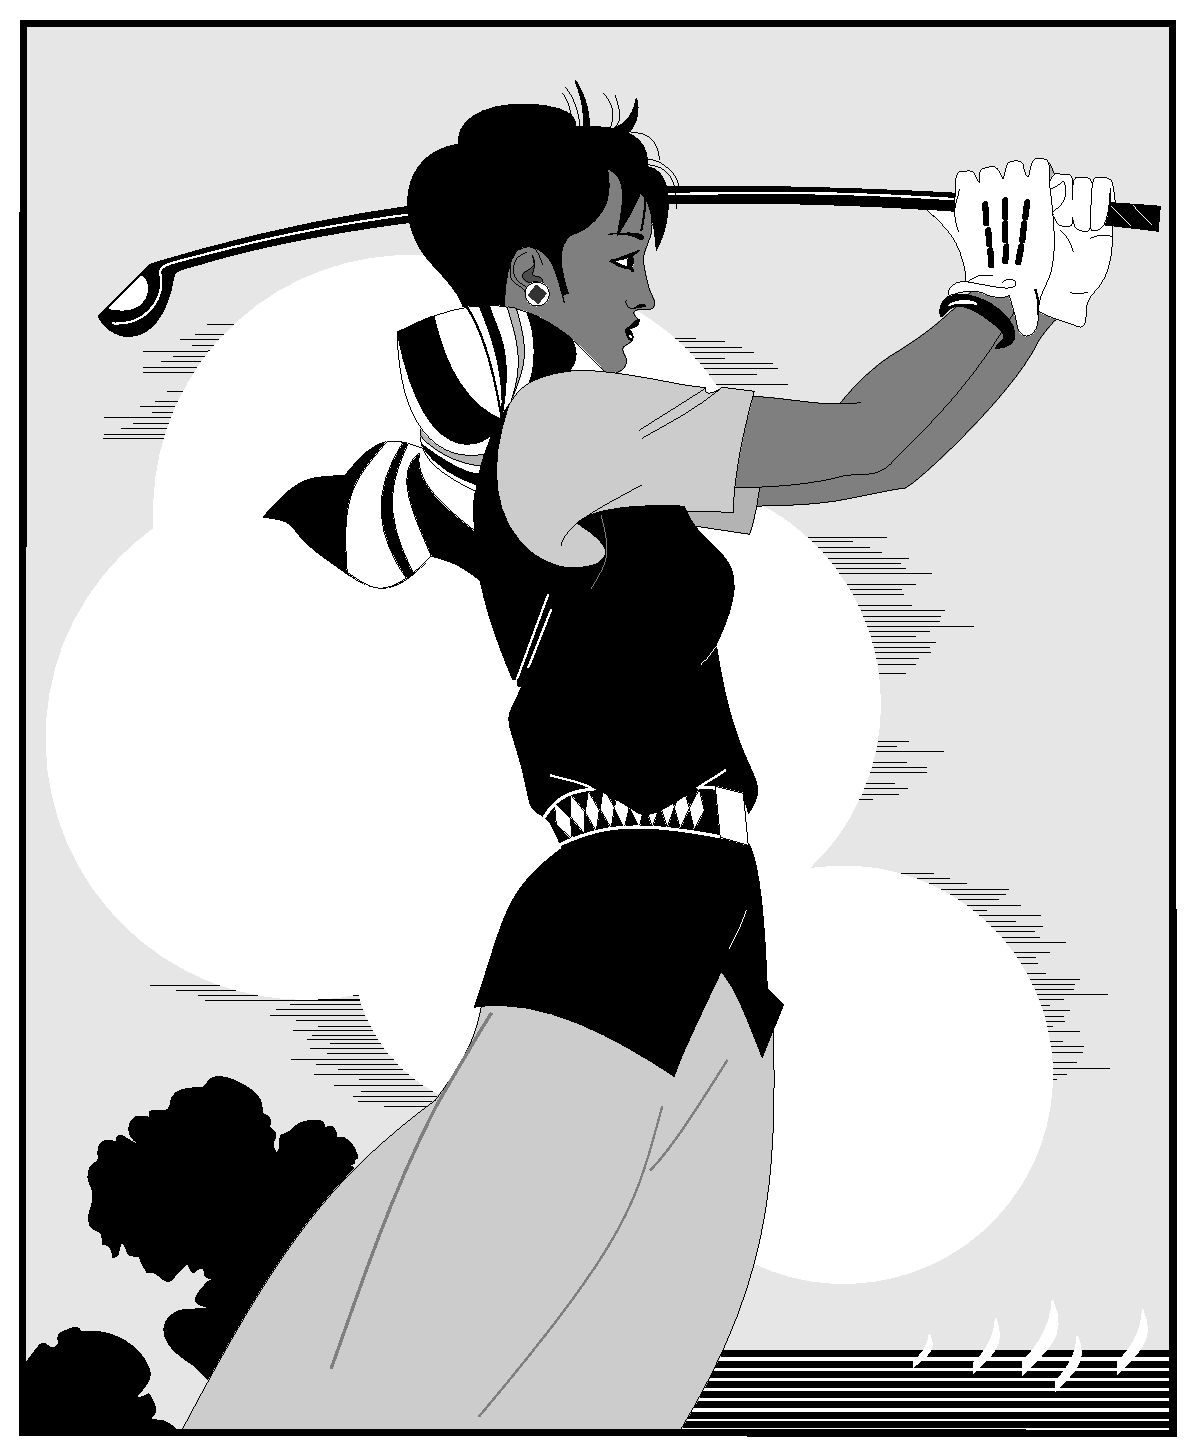
\includegraphics[width = 0.4\textwidth]{golfer}
\caption{打高尔夫球的人}
\label{fig:bm}
\end{figure}

\section{速度级运动学分析}

\subsection{并排图和子图}

位置级运动学的分析过程对速度级运动学的分析有很大帮助。在速度级运动学分析中,绳驱机械臂同样需要考虑三个空间,分别是驱动空间、关节空间以及操作空间。三者之间的关系如\figref{fig:parell1}与\figref{fig:parell2}所示。

\begin{figure}[htbp]
\centering
\begin{minipage}[t]{0.4\textwidth}
\centering
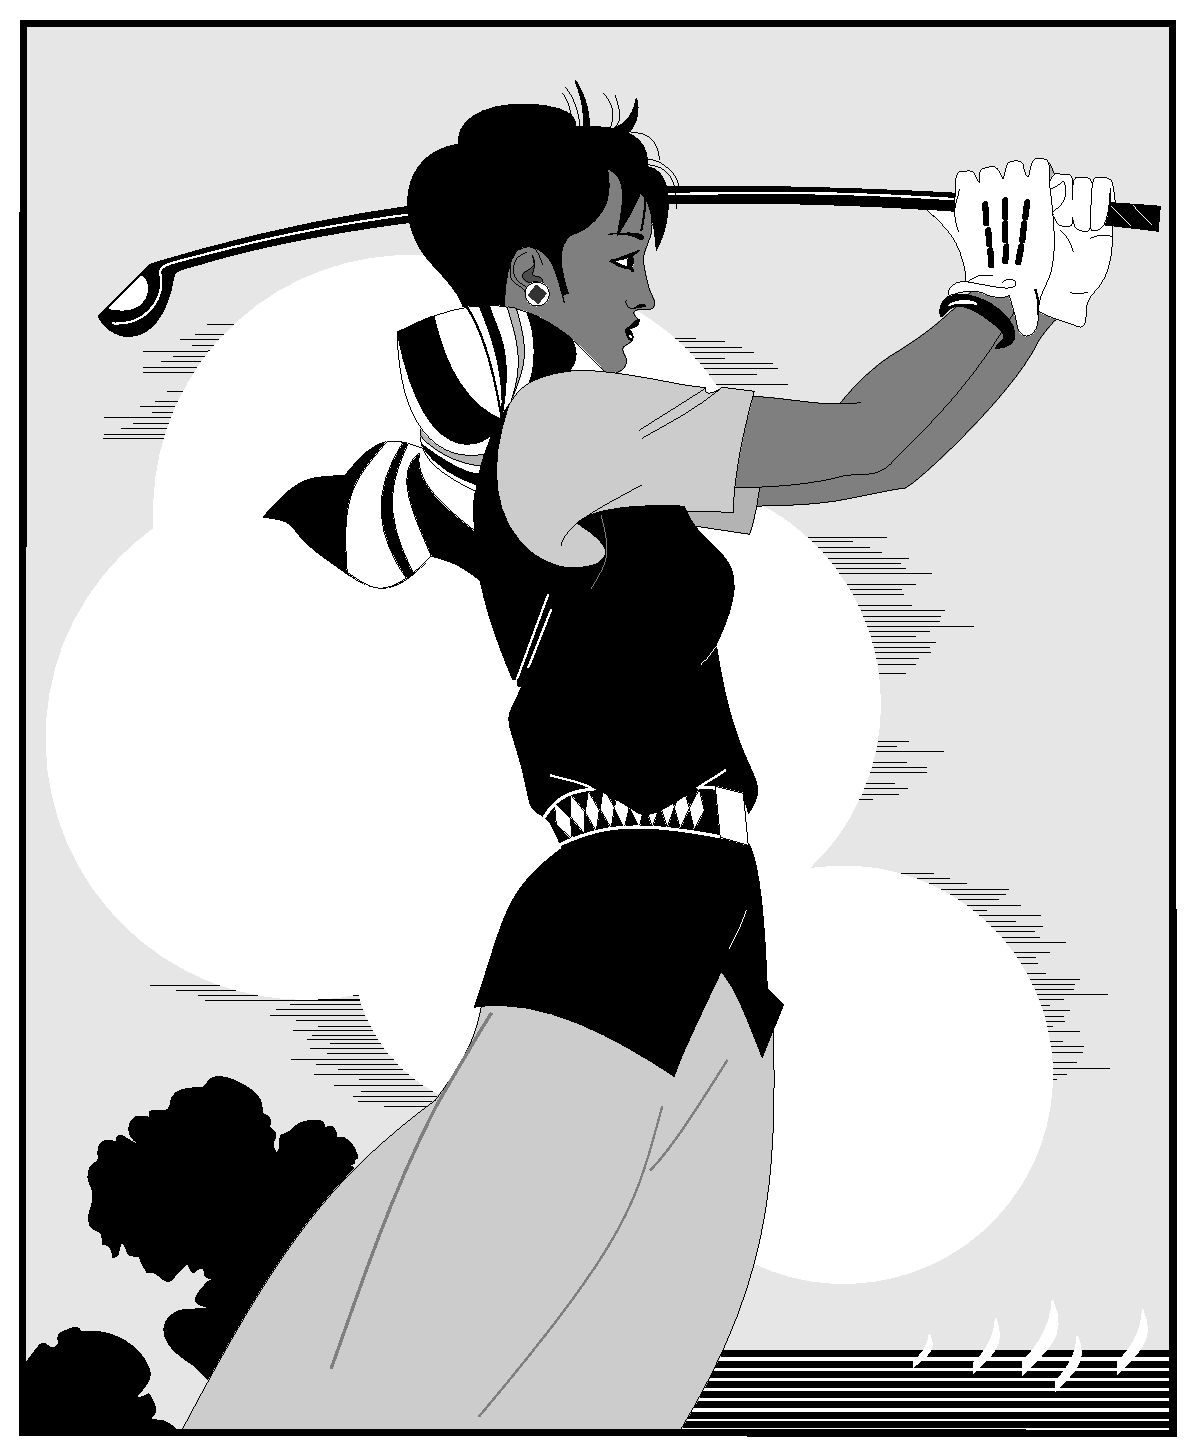
\includegraphics[width=\textwidth,height=\textwidth]{golfer}
\caption{打高尔夫球的人。注意,此图对齐方式是图片底部对齐}
\label{fig:parell1}
\end{minipage}
\centering
\begin{minipage}[t]{0.4\textwidth}
\centering
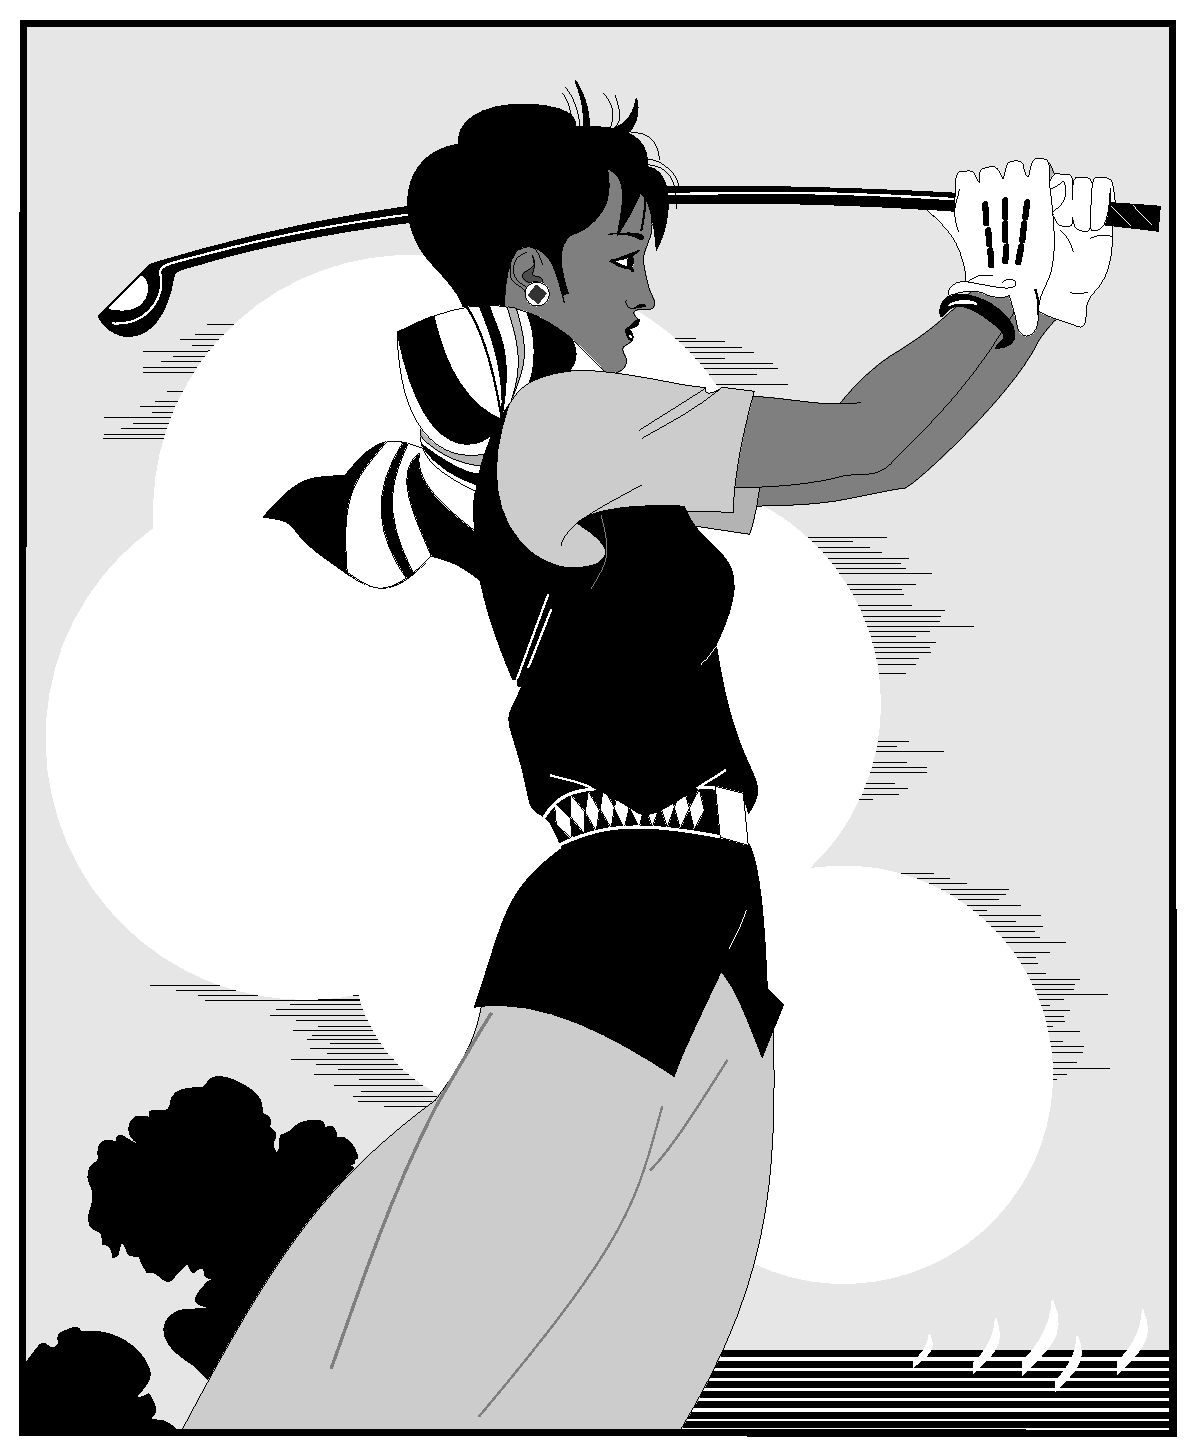
\includegraphics[width=\textwidth]{golfer}
\caption{打高尔夫球的人}
\label{fig:parell2}
\end{minipage}
\end{figure}

\section{本章小结}

总结本章的叙述内容。

\lipsum[1]


% 第3章
% !TEX root = ../main.tex

\chapter{内容XXX}

\section{引言}

每章的引言起到承接上一章引启下一章的作用。

\ldots\ldots

\section{对物理量符号进行注释的情况}

为使得对公式中物理量符号注释的转行与破折号“———”后第一个字对齐,此处最好采用表格环境。此表格无任何线条,左对齐,且在破折号处对齐,一共有“式中”二字、物理量符号和注释三列,表格的总宽度可选为文本宽度,因此应该采用\verb|tabularx|环境。由\verb|tabularx|环境生成的对公式中物理量符号进行注释的公式如式(\ref{eq:1})所示。
\begin{equation}\label{eq:1}
\ddot{\bm{\rho}}-\frac{\mu}{R_{t}^{3}}\left(3\bm{R_{t}}\frac{\bm{R_{t}\rho}}{R_{t}^{2}}-\bm{\rho}\right)=\bm{a}
\end{equation}
\begin{tabularx}{\textwidth}{@{}l@{\quad}r@{———}X@{}}
式中& $\bm{\rho}$ &追踪飞行器与目标飞行器之间的相对位置矢量;\\
&  $\bm{\ddot{\rho}}$&追踪飞行器与目标飞行器之间的相对加速度;\\
&  $\bm{a}$   &推力所产生的加速度;\\
&  $\bm{R_t}$ & 目标飞行器在惯性坐标系中的位置矢量;\\
&  $\omega_{t}$ & 目标飞行器的轨道角速度;\\
\end{tabularx}\vspace{3.15bp}
由此方法生成的注释内容应紧邻待注释公式并置于其下方,因此不能将代码放入\verb|table|浮动环境中。但此方法不能实现自动转页接排,可能会在当前页剩余空间不够时,全部移动到下一页而导致当前页出现很大空白。因此在需要转页处理时,还请您手动将需要转页的代码放入一个新的\verb|tabularx|环境中,将原来的一个\verb|tabularx|环境拆分为两个\verb|tabularx|环境。

{\color{red}(矩阵、矢量用“粗、斜体”,如矢量$\bm{R}$;单变量用“斜体”(不加粗),如$x,y$;上下标:有变量含义的用斜体,如$x_i$;数字、单词首字母、单位等无变量含义的用正体,如$x_1$,矩阵转置$\bm{A}^{\text{T}}$(T 为转置Transpose 的首字母))}

\section{子公式}

子公式编号示例:如果需要对公式的子公式进行编号,则使用\lstinline{subeqnarray}环境:
\begin{subeqnarray}
  \label{eqw}
  \slabel{eq0}
  x & = & a \times b \\
  \slabel{eq1}
  & = & z + t\\
  \slabel{eq2}
  & = & z + t
\end{subeqnarray}

\equref{eqw}中,\lstinline{label}为整个公式的标签,\lstinline{slabel}为子公式的标签。

\section{本章小结}

总结本章的叙述内容。

\lipsum[1]


% 第4章
% !TEX root = ../main.tex

\chapter{内容XXX}

\section{引言}

每章的引言起到承接上一章引启下一章的作用。

\ldots\ldots

\section{普通表格的绘制方法}

表格应具有三线表格式,因此需要调用~booktabs~宏包,其标准格式如表~\ref{table1}~所示。
\begin{table}[htbp]
\caption{符合研究生院绘图规范的表格}
\label{table1}
\vspace{0.5em}\centering\wuhao
\begin{tabular}{ccccc}
\toprule[1.5pt]
$D$(in) & $P_u$(lbs) & $u_u$(in) & $\beta$ & $G_f$(psi.in)\\
\midrule[1pt]
 5 & 269.8 & 0.000674 & 1.79 & 0.04089\\
10 & 421.0 & 0.001035 & 3.59 & 0.04089\\
20 & 640.2 & 0.001565 & 7.18 & 0.04089\\
\bottomrule[1.5pt]
\end{tabular}
\end{table}
全表如用同一单位,则将单位符号移至表头右上角,加圆括号。表中数据应准确无误,书写清楚。数字空缺的格内加横线“-”(占~2~个数字宽度)。表内文字或数字上、下或左、右相同时,采用通栏处理方式,不允许用“〃”、“同上”之类的写法。表内文字说明,起行空一格、转行顶格、句末不加标点。如某个表需要转页接排,在随后的各页上应重复表的编号。编号后加“(续表)”,表题可省略。续表应重复表头。

\section{XXXX分析}

\lipsum[1]

\section{XXXX分析}

\lipsum[2]

\section{本章小结}

总结本章的叙述内容。

\lipsum[3]


% 第5章
% !TEX root = ../main.tex

\chapter{内容XXX}

\section{引言}

每章的引言起到承接上一章引启下一章的作用。

\ldots\ldots

\section{参考文献引用方法}

\sindex[china]{du!段誉}引文标注遵照GB/T7714-2005,采用顺序编码制。正文中引用文献的标示应置于所引内容最后一个字的右上角,所引文献编号用阿拉伯数字置于方括号“[ ]”中,用小4号字体的上角标。要求:

(1)引用单篇文献时,如“二次铣削\cite{ren2010}”。

(2)同一处引用多篇文献时,各篇文献的序号在方括号内全部列出,各序号间用“,”,如
遇连续序号,可标注讫序号。如,…形成了多种数学模型\cite{Gravagne2003,ren2010}…
注意此处添加\cs{inlinecite}中文空格\inlinecite{Gravagne2003,ren2010},可以在cfg文件中修改空格类型。

(3)多次引用同一文献时,在文献序号的“[ ]”后标注引文页码。如,…间质细胞CAMP含量
测定\cite[100-197]{Gravagne2003}…。…含量测定方法规定
\cite[92]{Gravagne2003}…。

(4)当提及的参考文献为文中直接说明时,则用小4号字与正文排齐,如“由文献\inlinecite{webster2010}可知”

(5)多\cite{liu2016}引\cite{fu2018}用\cite{zhai2015}一\cite{yao2015}些\cite{jones2006}参\cite{mcmahan2005}考\cite{jones2004}文献以生成附录参考文献。

\section{XXXX分析}

\lipsum[1-2]

\section{本章小结}

总结本章的叙述内容。

\lipsum[1]


% 第6章
% !TEX root = ../main.tex

\chapter{内容XXX}

\section{引言}

每章的引言起到承接上一章引启下一章的作用。

\ldots\ldots

\section{定理和定义等}

\begin{theorem}[\cite{ren2010}]
宇宙大爆炸是一种爆炸。
\end{theorem}
\begin{definition}[(霍金)]
宇宙大爆炸是一种爆炸。
\end{definition}
\begin{assumption}
宇宙大爆炸是一种爆炸。
\end{assumption}
\begin{lemma}
宇宙大爆炸是一种爆炸。
\end{lemma}
\begin{corollary}
宇宙大爆炸是一种爆炸。
\end{corollary}
\begin{exercise}
宇宙大爆炸是一种爆炸。
\end{exercise}
\begin{problem}[(Albert Einstein)]
宇宙大爆炸是一种爆炸。
\end{problem}
\begin{remark}
宇宙大爆炸是一种爆炸。
\end{remark}
\begin{axiom}[(爱因斯坦)]
宇宙大爆炸是一种爆炸。
\end{axiom}
\begin{conjecture}
宇宙大爆炸是一种爆炸。
\end{conjecture}

\section{XXXX分析}

\subsection{算法}

算法不在规范中要求,此处不给出示例,在hitszthesis.sty中有定义示例。

\subsection{脚注}

不在再规范\footnote{规范是指\PGR\ 和\UGR}中要求,模板默认使用清华大学的格式。

\subsection{源码}

也不在再规范中要求。如果有需要最好使用minted包,但在编译的时候需要添加“-shell-escape”选项且安装pygmentize软件,这些不在模板中默认载入,如果需要自行载入。

\section{本章小结}

总结本章的叙述内容。

\lipsum[3]


% 开始写正文之后的部分
\backmatter

% 结论
% !TEX root = ../main.tex

% 结论
\begin{conclusions}

学位论文的结论作为论文正文的最后一章单独排写,但不加章标题序号。

结论是对整个论文主要成果的总结。在结论中应明确指出本研究内容的创新性成果或创新点(含新见解、新观点),并指出今后进一步在本研究方向进行研究工作的展望与设想,上述各项用(1).(2).  表述,不要将结论写成论文的摘要。结论字数一般在2000字以内。

\end{conclusions}


% 参考文献
\bibliographystyle{hitszthesis}
\bibliography{reference}

% 授权
\authorization

% 授权页为扫描的PDF文件(scan.pdf),与上面的命令互斥
% \authorization[scan.pdf]

% 致谢
% !TEX root = ../main.tex

% 致谢
\begin{acknowledgements}

对导师和给予指导或协助完成学位论文工作的组织和个人,对课题给予资助者表示感谢。内容应简朴、语言应含蓄。

衷心感谢导师XXX教授对本人的精心指导。$\cdots\cdots$,他的言传身教将使我终生受益。

感谢XXX教授,以及实验室全体老师和同窗们的热情帮助和支持!

本课题承蒙XXXX基金资助,特此致谢。

\end{acknowledgements}


% 附录
\begin{appendix}
  % !TEX root = ../main.tex

% 附录1
\chapter{外文资料的调研阅读报告或书面翻译}

\title{英文资料的中文标题}

{\heiti 摘要:} 本章为外文资料翻译内容。如果有摘要可以直接写上来,这部分好像没有
明确的规定。

\section{单目标规划}
北冥有鱼,其名为鲲。鲲之大,不知其几千里也。化而为鸟,其名为鹏。鹏之背,不知其几
千里也。怒而飞,其翼若垂天之云。是鸟也,海运则将徙于南冥。南冥者,天池也。
\begin{equation}\tag*{(123)}
 p(y|\mathbf{x}) = \frac{p(\mathbf{x},y)}{p(\mathbf{x})}=
\frac{p(\mathbf{x}|y)p(y)}{p(\mathbf{x})}
\end{equation}

吾生也有涯,而知也无涯。以有涯随无涯,殆已!已而为知者,殆而已矣!为善无近名,为
恶无近刑,缘督以为经,可以保身,可以全生,可以养亲,可以尽年。

\subsection{线性规划}
庖丁为文惠君解牛,手之所触,肩之所倚,足之所履,膝之所倚,砉然响然,奏刀騞然,莫
不中音,合于桑林之舞,乃中经首之会。
\begin{table}[ht]
\centering
  \centering
  \caption*{表~1\hskip1em 这是手动编号但不出现在索引中的一个表格例子}
  \label{tab:badtabular3}
  \begin{tabular}[c]{|m{1.5cm}|c|c|c|c|c|c|}\hline
    \multicolumn{2}{|c|}{Network Topology} & \# of nodes &
    \multicolumn{3}{c|}{\# of clients} & Server \\\hline
    GT-ITM & Waxman Transit-Stub & 600 &
    \multirow{2}{2em}{2\%}&
    \multirow{2}{2em}{10\%}&
    \multirow{2}{2em}{50\%}&
    \multirow{2}{1.2in}{Max. Connectivity}\\\cline{1-3}
    \multicolumn{2}{|c|}{Inet-2.1} & 6000 & & & &\\\hline
    & \multicolumn{2}{c|}{ABCDEF} &\multicolumn{4}{c|}{} \\\hline
\end{tabular}
\end{table}

文惠君曰:“嘻,善哉!技盖至此乎?”庖丁释刀对曰:“臣之所好者道也,进乎技矣。始臣之
解牛之时,所见无非全牛者;三年之后,未尝见全牛也;方今之时,臣以神遇而不以目视,
官知止而神欲行。依乎天理,批大郤,导大窾,因其固然。技经肯綮之未尝,而况大坬乎!
良庖岁更刀,割也;族庖月更刀,折也;今臣之刀十九年矣,所解数千牛矣,而刀刃若新发
于硎。彼节者有间而刀刃者无厚,以无厚入有间,恢恢乎其于游刃必有余地矣。是以十九年
而刀刃若新发于硎。虽然,每至于族,吾见其难为,怵然为戒,视为止,行为迟,动刀甚微,
謋然已解,如土委地。提刀而立,为之而四顾,为之踌躇满志,善刀而藏之。”

文惠君曰:“善哉!吾闻庖丁之言,得养生焉。”


\subsection{非线性规划}
孔子与柳下季为友,柳下季之弟名曰盗跖。盗跖从卒九千人,横行天下,侵暴诸侯。穴室枢
户,驱人牛马,取人妇女。贪得忘亲,不顾父母兄弟,不祭先祖。所过之邑,大国守城,小
国入保,万民苦之。孔子谓柳下季曰:“夫为人父者,必能诏其子;为人兄者,必能教其弟。
若父不能诏其子,兄不能教其弟,则无贵父子兄弟之亲矣。今先生,世之才士也,弟为盗
跖,为天下害,而弗能教也,丘窃为先生羞之。丘请为先生往说之。”

柳下季曰:“先生言为人父者必能诏其子,为人兄者必能教其弟,若子不听父之诏,弟不受
兄之教,虽今先生之辩,将奈之何哉?且跖之为人也,心如涌泉,意如飘风,强足以距敌,
辩足以饰非。顺其心则喜,逆其心则怒,易辱人以言。先生必无往。”

孔子不听,颜回为驭,子贡为右,往见盗跖。

\subsection{整数规划}
盗跖乃方休卒徒大山之阳,脍人肝而餔之。孔子下车而前,见谒者曰:“鲁人孔丘,闻将军
高义,敬再拜谒者。”谒者入通。盗跖闻之大怒,目如明星,发上指冠,曰:“此夫鲁国之
巧伪人孔丘非邪?为我告之:尔作言造语,妄称文、武,冠枝木之冠,带死牛之胁,多辞缪
说,不耕而食,不织而衣,摇唇鼓舌,擅生是非,以迷天下之主,使天下学士不反其本,妄
作孝弟,而侥幸于封侯富贵者也。子之罪大极重,疾走归!不然,我将以子肝益昼餔之膳。”
  % !TEX root = ../main.tex

% 附录2
\chapter{外文资料原文}
\label{cha:engorg}

\title{The title of the English paper}

\textbf{Abstract:} As one of the most widely used techniques in operations
research, \emph{ mathematical programming} is defined as a means of maximizing a
quantity known as \emph{bjective function}, subject to a set of constraints
represented by equations and inequalities. Some known subtopics of mathematical
programming are linear programming, nonlinear programming, multiobjective
programming, goal programming, dynamic programming, and multilevel
programming$^{[1]}$.

It is impossible to cover in a single chapter every concept of mathematical
programming. This chapter introduces only the basic concepts and techniques of
mathematical programming such that readers gain an understanding of them
throughout the book$^{[2,3]}$.


\section{Single-Objective Programming}
The general form of single-objective programming (SOP) is written
as follows,
\begin{equation}\tag*{(123)} % 如果附录中的公式不想让它出现在公式索引中,那就请
                             % 用 \tag*{xxxx}
\left\{\begin{array}{l}
\max \,\,f(x)\\[0.1 cm]
\mbox{subject to:} \\ [0.1 cm]
\qquad g_j(x)\le 0,\quad j=1,2,\cdots,p
\end{array}\right.
\end{equation}
which maximizes a real-valued function $f$ of
$x=(x_1,x_2,\cdots,x_n)$ subject to a set of constraints.

\newtheorem{mpdef}{Definition}[chapter]
\begin{mpdef}
In SOP, we call $x$ a decision vector, and
$x_1,x_2,\cdots,x_n$ decision variables. The function
$f$ is called the objective function. The set
\begin{equation}\tag*{(456)} % 这里同理,其它不再一一指定。
S=\left\{x\in\Re^n\bigm|g_j(x)\le 0,\,j=1,2,\cdots,p\right\}
\end{equation}
is called the feasible set. An element $x$ in $S$ is called a
feasible solution.
\end{mpdef}

\newtheorem{mpdefop}[mpdef]{Definition}
\begin{mpdefop}
A feasible solution $x^*$ is called the optimal
solution of SOP if and only if
\begin{equation}
f(x^*)\ge f(x)
\end{equation}
for any feasible solution $x$.
\end{mpdefop}

One of the outstanding contributions to mathematical programming was known as
the Kuhn-Tucker conditions\ref{eq:ktc}. In order to introduce them, let us give
some definitions. An inequality constraint $g_j(x)\le 0$ is said to be active at
a point $x^*$ if $g_j(x^*)=0$. A point $x^*$ satisfying $g_j(x^*)\le 0$ is said
to be regular if the gradient vectors $\nabla g_j(x)$ of all active constraints
are linearly independent.

Let $x^*$ be a regular point of the constraints of SOP and assume that all the
functions $f(x)$ and $g_j(x),j=1,2,\cdots,p$ are differentiable. If $x^*$ is a
local optimal solution, then there exist Lagrange multipliers
$\lambda_j,j=1,2,\cdots,p$ such that the following Kuhn-Tucker conditions hold,
\begin{equation}
\label{eq:ktc}
\left\{\begin{array}{l}
    \nabla f(x^*)-\sum\limits_{j=1}^p\lambda_j\nabla g_j(x^*)=0\\[0.3cm]
    \lambda_jg_j(x^*)=0,\quad j=1,2,\cdots,p\\[0.2cm]
    \lambda_j\ge 0,\quad j=1,2,\cdots,p.
\end{array}\right.
\end{equation}
If all the functions $f(x)$ and $g_j(x),j=1,2,\cdots,p$ are convex and
differentiable, and the point $x^*$ satisfies the Kuhn-Tucker conditions
(\ref{eq:ktc}), then it has been proved that the point $x^*$ is a global optimal
solution of SOP.

\subsection{Linear Programming}
\label{sec:lp}

If the functions $f(x),g_j(x),j=1,2,\cdots,p$ are all linear, then SOP is called
a {\em linear programming}.

The feasible set of linear is always convex. A point $x$ is called an extreme
point of convex set $S$ if $x\in S$ and $x$ cannot be expressed as a convex
combination of two points in $S$. It has been shown that the optimal solution to
linear programming corresponds to an extreme point of its feasible set provided
that the feasible set $S$ is bounded. This fact is the basis of the {\em simplex
  algorithm} which was developed by Dantzig as a very efficient method for
solving linear programming.
\begin{table}[ht]
\centering
  \centering
  \caption*{Table~1\hskip1em This is an example for manually numbered table, which
    would not appear in the list of tables}
  \label{tab:badtabular2}
  \begin{tabular}[c]{|m{1.5cm}|c|c|c|c|c|c|}\hline
    \multicolumn{2}{|c|}{Network Topology} & \# of nodes &
    \multicolumn{3}{c|}{\# of clients} & Server \\\hline
    GT-ITM & Waxman Transit-Stub & 600 &
    \multirow{2}{2em}{2\%}&
    \multirow{2}{2em}{10\%}&
    \multirow{2}{2em}{50\%}&
    \multirow{2}{1.2in}{Max. Connectivity}\\\cline{1-3}
    \multicolumn{2}{|c|}{Inet-2.1} & 6000 & & & &\\\hline
    & \multicolumn{2}{c|}{ABCDEF} &\multicolumn{4}{c|}{} \\\hline
\end{tabular}
\end{table}

Roughly speaking, the simplex algorithm examines only the extreme points of the
feasible set, rather than all feasible points. At first, the simplex algorithm
selects an extreme point as the initial point. The successive extreme point is
selected so as to improve the objective function value. The procedure is
repeated until no improvement in objective function value can be made. The last
extreme point is the optimal solution.

\subsection{Nonlinear Programming}

If at least one of the functions $f(x),g_j(x),j=1,2,\cdots,p$ is nonlinear, then
SOP is called a {\em nonlinear programming}.

A large number of classical optimization methods have been developed to treat
special-structural nonlinear programming based on the mathematical theory
concerned with analyzing the structure of problems.

Now we consider a nonlinear programming which is confronted solely with
maximizing a real-valued function with domain $\Re^n$.  Whether derivatives are
available or not, the usual strategy is first to select a point in $\Re^n$ which
is thought to be the most likely place where the maximum exists. If there is no
information available on which to base such a selection, a point is chosen at
random. From this first point an attempt is made to construct a sequence of
points, each of which yields an improved objective function value over its
predecessor. The next point to be added to the sequence is chosen by analyzing
the behavior of the function at the previous points. This construction continues
until some termination criterion is met. Methods based upon this strategy are
called {\em ascent methods}, which can be classified as {\em direct methods},
{\em gradient methods}, and {\em Hessian methods} according to the information
about the behavior of objective function $f$. Direct methods require only that
the function can be evaluated at each point. Gradient methods require the
evaluation of first derivatives of $f$. Hessian methods require the evaluation
of second derivatives. In fact, there is no superior method for all
problems. The efficiency of a method is very much dependent upon the objective
function.

\subsection{Integer Programming}

{\em Integer programming} is a special mathematical programming in which all of
the variables are assumed to be only integer values. When there are not only
integer variables but also conventional continuous variables, we call it {\em
  mixed integer programming}. If all the variables are assumed either 0 or 1,
then the problem is termed a {\em zero-one programming}. Although integer
programming can be solved by an {\em exhaustive enumeration} theoretically, it
is impractical to solve realistically sized integer programming problems. The
most successful algorithm so far found to solve integer programming is called
the {\em branch-and-bound enumeration} developed by Balas (1965) and Dakin
(1965). The other technique to integer programming is the {\em cutting plane
  method} developed by Gomory (1959).

\hfill\textit{Uncertain Programming\/}\quad(\textsl{BaoDing Liu, 2006.2})

\section*{References}
\noindent{\itshape NOTE: These references are only for demonstration. They are
  not real citations in the original text.}

\begin{translationbib}
\item Donald E. Knuth. The \TeX book. Addison-Wesley, 1984. ISBN: 0-201-13448-9
\item Paul W. Abrahams, Karl Berry and Kathryn A. Hargreaves. \TeX\ for the
  Impatient. Addison-Wesley, 1990. ISBN: 0-201-51375-7
\item David Salomon. The advanced \TeX book.  New York : Springer, 1995. ISBN:0-387-94556-3
\end{translationbib}

  % !TEX root = ../main.tex

% 附录3
\chapter{其它附录}

不论何种类型的论文都要将其中一篇与所撰写论文内容最直接相关的外文文献译成中文,不少于3000汉字,并将其编入附录。有些不宜放在正文中,但有参考价值的内容(如外文文献复印件及中文译文、公式的推导、程序流程图、图纸、数据表格等)可编入论文的附录中。附录放在论文最后,如不宜放在论文后面时可单独装订,与论文一起保存。

附录1与附录2为外文文献翻译示例,其他的附录如数据、代码等,可以放在这里。

\end{appendix}


% 结束文档撰写
\end{document}
%%=============================================

% Local Variables:
% TeX-engine: xetex
% End:
